\section{Durchführung und Aufbau}
\label{sec:Durchführung}
Ziel des Versuches ist es sich mit de Grundlagen der Vakuumtechnik vertraut zu machen und das Saugvermögen sowie die Leckrate von einer Drehschiebepumpe als auch einer Trubopumpe zu bestimmen. Eine Skizze des Aufbaus ist in Abbildung \ref{??} zu sehen. 
\begin{figure}[htpb]
  \centering
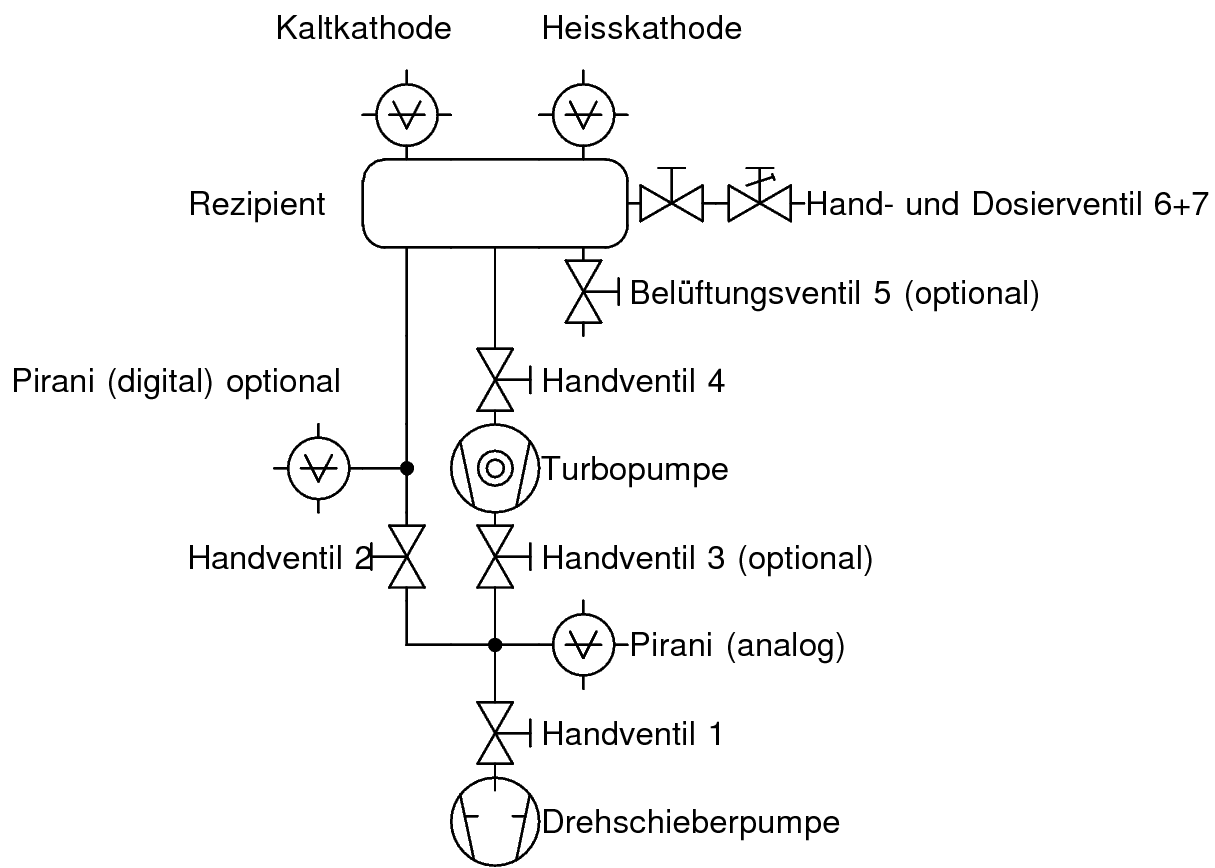
\includegraphics[width=0.8\textwidth]{picture/pumpaufbau.png}
  \caption{Schema des Aufbaus des Pumpstandes}
  \label{fig:pump}
\end{figure}
Beim Aufbau des Vakuumstandes wurde darauf geachtet das Volumen des System möglichst gering zu halten um das System übersichtlich zu halten. Alle Dichtungen sind Handfest zugezogen und der Rezipient erwärmt worden um das Ausgasen zu verrringern. \newline
Zunächst soll die p(t)-Kurve aufgenommen werde. Dafür wurde der Pumpstand wie in Abbildung \ref{fig:Dreh} zu sehen aufgebaut. 
\begin{figure}[htpb]
  \centering
  \includegraphics[width=\textwidth]{picture/Aufbau1.png}
  \caption{Pumpstand zur Bestimmung der Kennziffern der Drehschieberpumpe}
  \label{fig:Dreh}
\end{figure}
Als erstes wird dafür der Maximaldruck der Drehschieberpumpe gemessen. Dazu muss das Überdruckventil (3 \& 4) geschlossen werden und der Druck durch die analoge Anzeige des Pirani-Messgerät(7) abgelse werden. Anschließend wird für 4 verschiedene Drücke jeweils zu 18 verschiedenen Drücken die Zeit genommen welche die Pumpe benötigt um diese zu errreichen. Die Messreihe wird jeweils 3-mal durchgeführt. 
Anschließend wird die Leckrate bestimmt indem die Leckrate 

\begin{figure}[htpb]
  \centering
  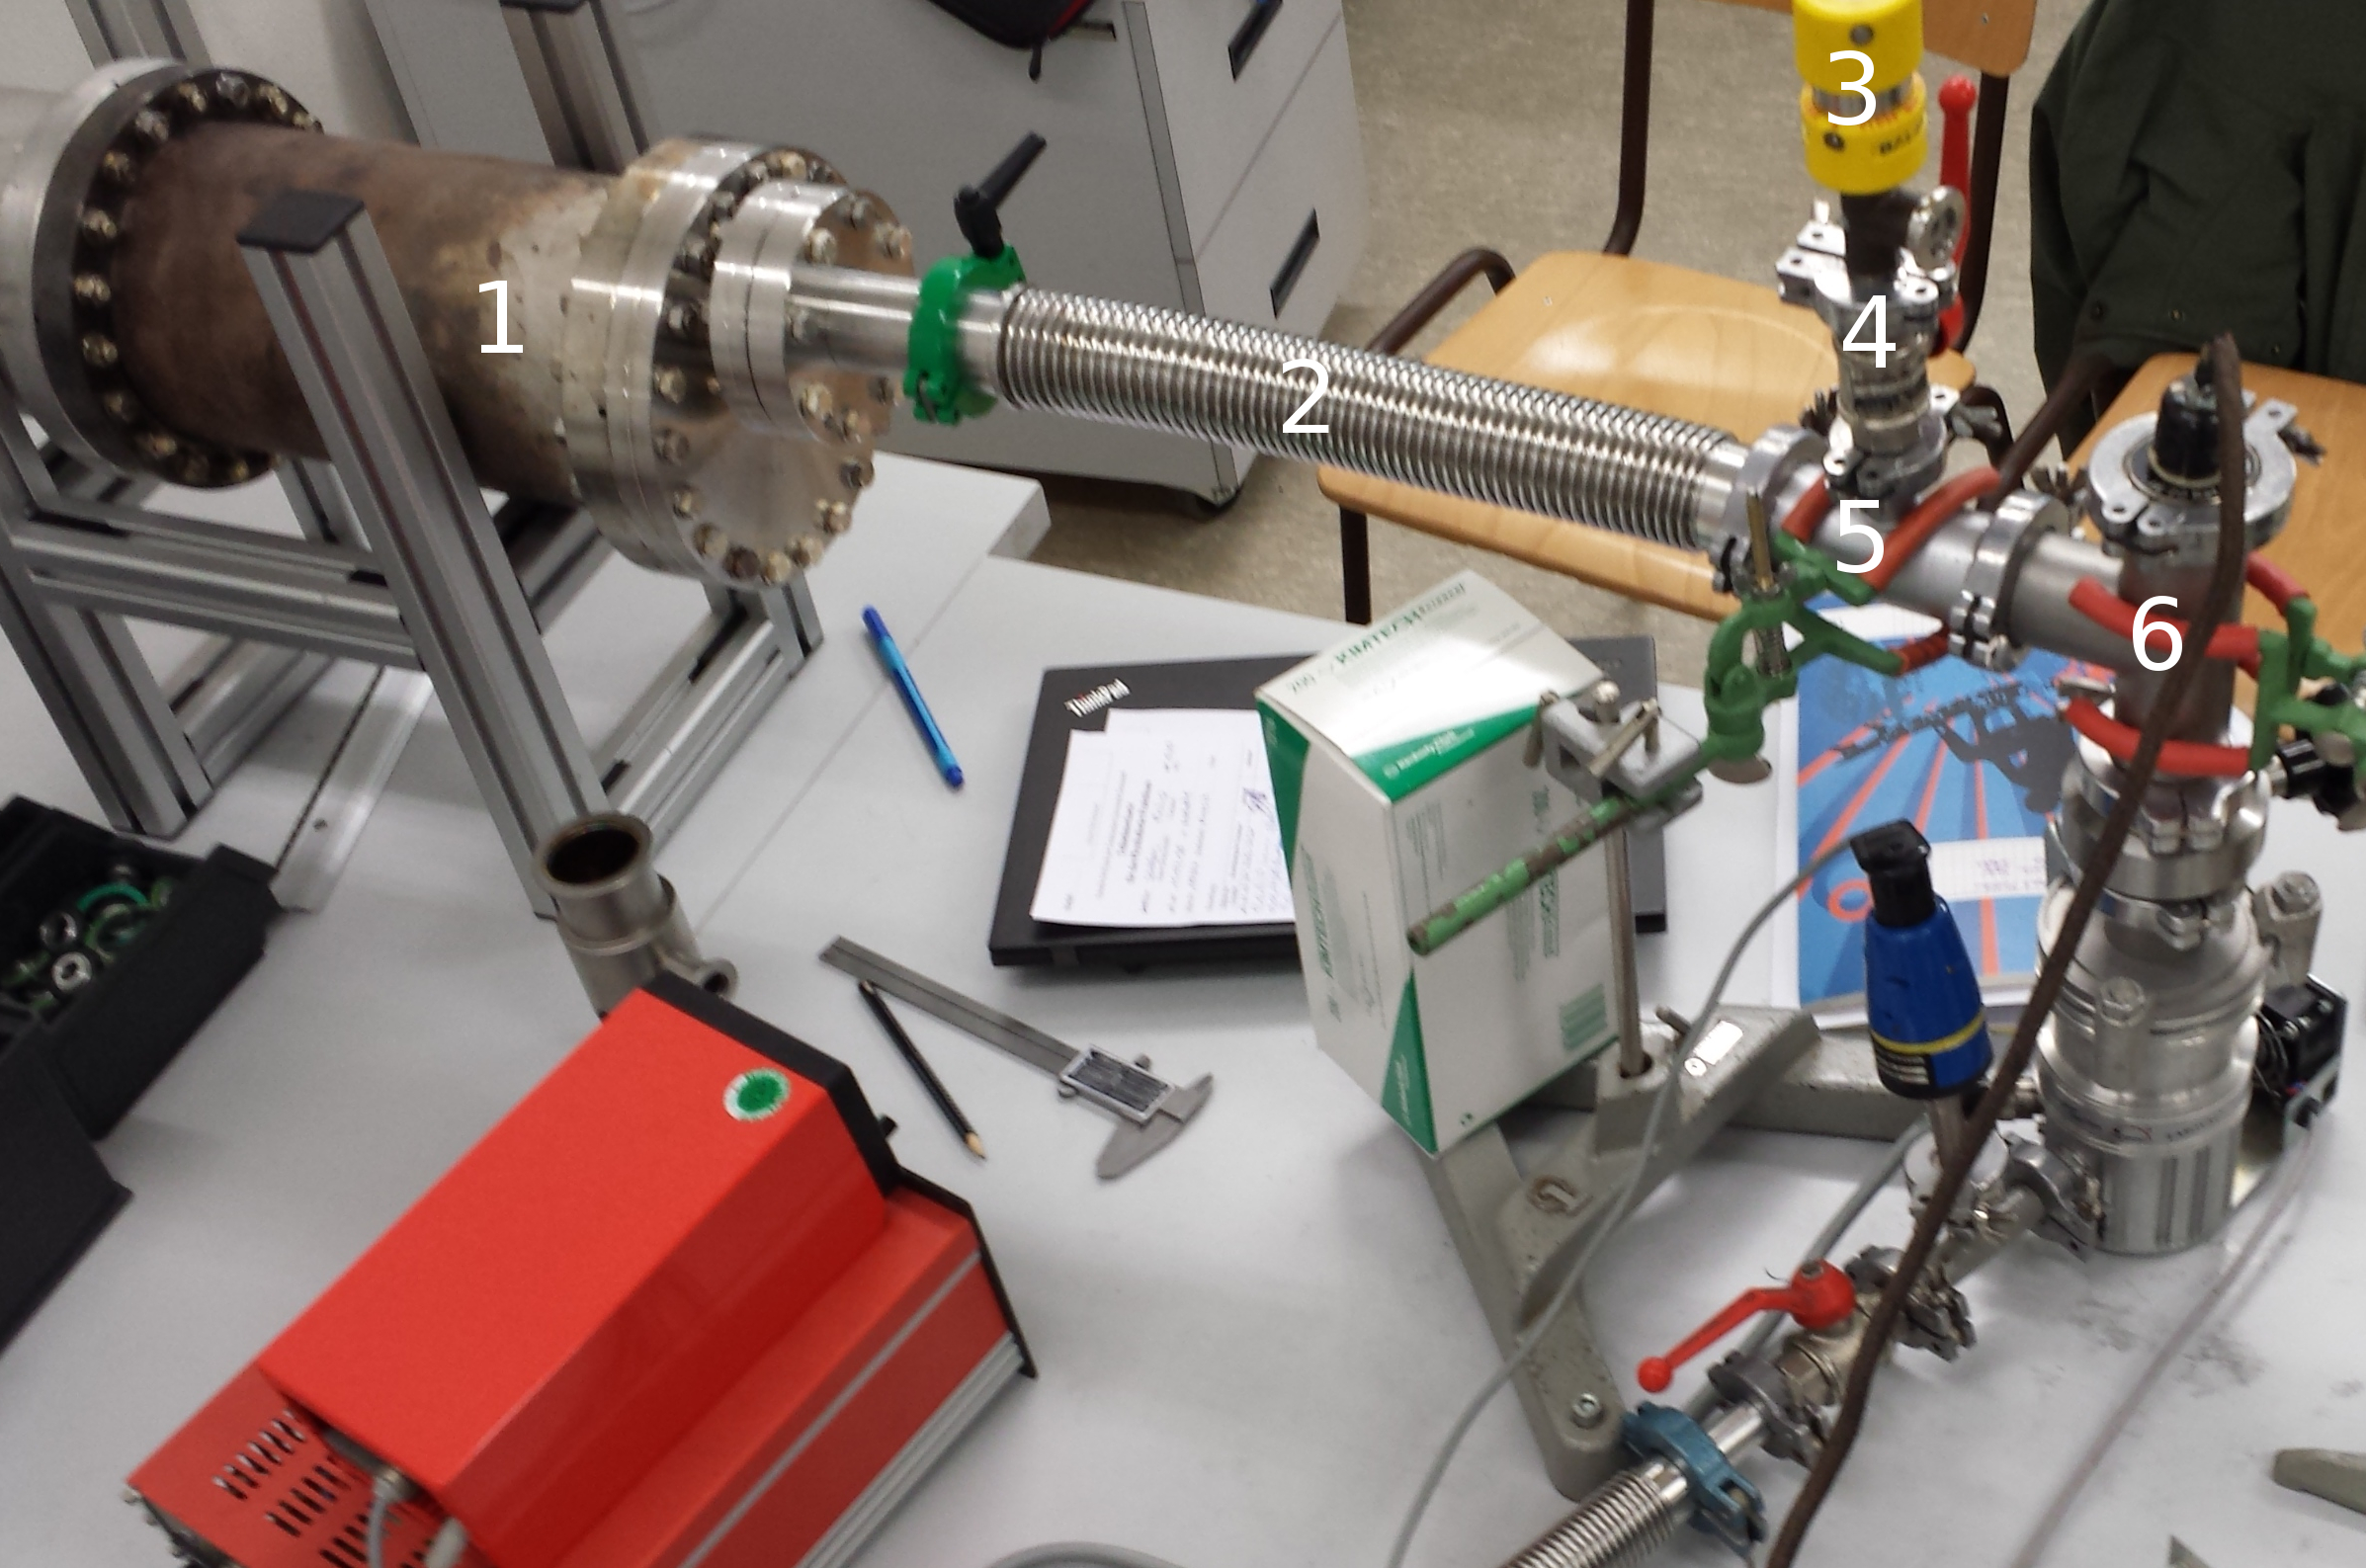
\includegraphics[width=\textwidth]{picture/Aufgabe2.png}
  \caption{<+caption text+>}
  \label{fig:<+label+>}
\end{figure}<++>
